\subsection{Sofware environment}
\label{subsec:3.1}
The software environment on Monch  and Pilatus is controlled using the
modules framework which gives an easy and flexible mechanism to access
to all of the CSCS  provided compilers, tools and applications.  It is
particularly  useful for  testing code  portability  between different
compilers  or for  changing  between different  versions  of the  same
compiler.  INT2LM  and the COSMO-ART model are  implemented in Fortran
90 for distributed memory parallel computers using the Message Passing
Interface (MPI).  For  our initial benchmarking, we opted  for the GNU
compiler  (gcc/4.8.1 on  Monch,  gcc/4.8.2 on  Pilatus)  with the  -O3
compiler flag as  it generally gives a good  level of optimization and
the code runs faster in this configuration than when compiled with the
intel compiler  (intel/14.0.1), also available on  Monch.  Besides, we
installed the  MPICH2 implementation of MPI (mvapich2/1.9)  as well as
the  commonly  used   HDF5  (hdf5/1.8.12)  and  NetCDF  (netcdf/4.3.1)
libraries in favor of the  traditional GRIB library for the management
of  extremely  large and  complex  data  collections.   Note that  all
compute  nodes of  Monch  and Pilatus  used  respectively the  ``Linux
2.6.32-358.11.1.el6.x86\_64''   and   ``Linux   3.0.101-0.15-default''
operating systems.

\subsection{Run configuration}
\label{subsec:3.2}
The COSMO-ART model uses NAMELIST-input to specify runtime parameters
splitted into several groups:

\begin{itemize}
\item LMGRID: specifying the domain and the size of the grid,
\item RUNCTL: parameters for the model run,
\item TUNING: parameters for tuning physics and dynamics,
\item DYNCTL: parameters for the adiabatic model,
\item PHYCTL: parameters for the diabatic model,
\item COSMO\_ART: parameters for gases and aerosols model,
\item DIACTL: parameters for the diagnostic calculations,
\item SATCTL: controlling computation of synthetic satellite images,
\item IOCTL: controlling the I/O environment,
\item GRIBIN: controlling the grib input,
\item GRIBOUT: controlling the grib output,
\end{itemize}

\noindent
To run COSMO-ART the following input data are necessary:
\begin{itemize}
\item  Gas phase:  Anthropogenic emissions  for different  species and
  land use data for biogenic emissions and deposition,
\item Aerosol particles: Anthropogenic emissions,
\item Mineral dust: Soil specific land use data.
\end{itemize}

A snapshot of the code, which includes, at least conceptually, all the
information needed  to reproduce the  energy-to-solution benchmarks of
COSMO-ART, was  produced and run on a  full rack of 52  nodes on Monch
(monchc[029-080]), i.e.  a total of 1040 cores using 20 tasks per node
and on  a full rack of  42 nodes on Pilatus  (pilatus[03-44]), i.e.  a
total of  1344 cores using 16  tasks per node.   The calculated region
was  mapped to  the participating  processors using  a 2D-partitioning
strategy.  The distribution along the  x and y coordinates was defined
by setting: $nprocx=40$ and  $nprocy=26$ for Monch and $nprocx=28$ and
$nprocy=24$.  Besides as this version of COSMO-ART doesn't make use of
the   GRIB   library,  we   specified   $nprocio=0$   for  GRIB   I/O.
Hyperthreading is not considered in this study as previous attempts of
its use revealed that it always led to higher energy-to-solution.\\

Multiple production runs of COSMO-ART were performed to illustrate the
reproducibility  of   the  baseline,  and   quantify  the  significant
uncertainties in  the power measurement, as dictated  by the available
technology (see subsection~\ref{subsec:2.2}).

\subsection{Power-measurement results}
\label{subsec:3.3}
Measuring  the power  consumption on  one entire  Cray cabinet  is the
easiest    way    to    calculate   energy-to-solution    for    given
applications.  The total  energy  to solution  is the  straightforward
calculation:\\

Energy-to-solution  =  Integral  of  power consumption  over  the  job
duration\\

However, the average power consumption times the job duration is often
sufficient.

\subsubsection{Monch (CSCS - ETH Zurich)}
\begin{figure*}
  \includegraphics[width=0.4\textwidth]{Figs/NRJ_benchmark_Monch.eps}
  \caption{Isola E1 Rack 2 Total Power and Isola E1 Total Power}
  \label{fig:1}
\end{figure*}

The 1-day simulation was issued successfully twice, the start time and
execution time for both runs are:
\begin{itemize}
\item start=12:51:03, end=13:20:46 $\Rightarrow$ T = 00:29:43 = 1783 s
\item start=14:28:40, end=14:58:02 $\Rightarrow$ T = 00:29:22 = 1762 s
\end{itemize}

The power  consumption for  both jobs is  calculated by  averaging the
corresponding power  measurements from the Excel  file.  Power results
account for the  Isola E1 Rack 2 Total Power. As  time resolution is 5
minutes  for the  output  results, the  average  power consumption  is
computed   by  considering  6   values  for   each  single   run  (see
Table~\ref{tab:1}).

\begin{table}
  \begin{center}
    \caption{}
    \label{tab:1}
    \begin{tabular}{lll}
      \hline\noalign{\smallskip}
      Time & Measured power (W) & Average power (W)  \\
      \noalign{\smallskip}\hline\noalign{\smallskip}
      12:55:00 & 1.2355833333e+04 & 1.265852278e+04 \\ 
      13:00:00 & 1.2820266667e+04 &  \\
      13:05:00 & 1.2600743333e+04 &  \\ 
      13:10:00 & 1.2811580000e+04 &  \\
      13:15:00 & 1.2609680000e+04 &  \\
      13:20:00 & 1.2753033333e+04 &  \\
      \noalign{\smallskip}\hline\noalign{\smallskip}
      14:30:00 & 1.2019266667e+04 & 1.258640833e+04 \\ 
      14:35:00 & 1.2632253333e+04 &  \\
      14:40:00 & 1.2779040000e+04 &  \\
      14:45:00 & 1.2753180000e+04 &  \\
      14:50:00 & 1.2610476667e+04 &  \\
      14:55:00 & 1.2724233333e+04 &  \\
      \noalign{\smallskip}\hline
    \end{tabular}
  \end{center}
\end{table}

Thus, the total energy consumption corresponds to: 
\begin{itemize}
\item E  = 1783 x 12658.52278  = 22570146.11674 J $\sim$  22.57 MJ per
  day of simulation
\item E  = 1762 x 12586.40833  = 22177251.47746 J $\sim$  22.18 MJ per
  day of simulation
\end{itemize}

\subsubsection{Pilatus (CSCS - ETH Zurich)}
\begin{figure*}
  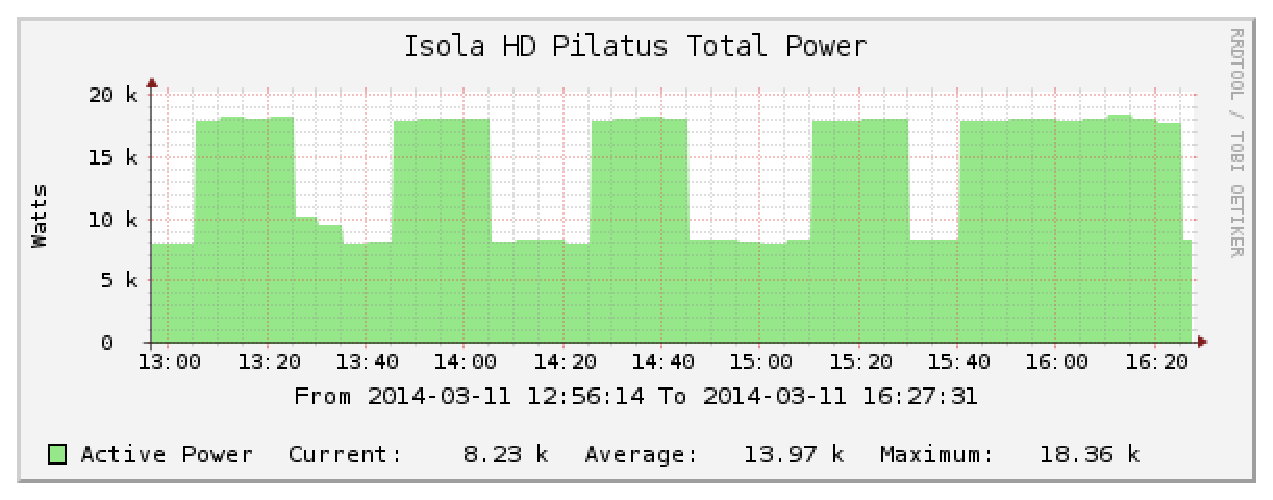
\includegraphics[width=0.4\textwidth]{Figs/NRJ_benchmark_Pilatus.eps}
  \caption{Isola HD Pilatus Total Power}
  \label{fig:2}
\end{figure*}

The 1-day simulation was issued successfully four times and the 2-days
run only once, the start time and execution time for all jobs are:
\begin{itemize}
\item start=13:07:25, end=13:29:47 $\Rightarrow$ T = 00:22:22 = 1342 s
\item start=13:46:04, end=14:08:30 $\Rightarrow$ T = 00:22:26 = 1346 s
\item start=14:27:51, end=14:50:01 $\Rightarrow$ T = 00:22:10 = 1330 s
\item start=15:10:04, end=15:32:17 $\Rightarrow$ T = 00:22:13 = 1333 s
\item start=15:41:48, end=16:26:13 $\Rightarrow$ T = 00:44:25 = 2665 s
\end{itemize}

Again, the power  consumption for all jobs is  calculated by averaging
the  corresponding  power  measurements  from the  Excel  file.  Power
results  account  for  the  Isola  HD Pilatus  Total  Power.  As  time
resolution  is 5  minutes for  the output  results, the  average power
consumption is computed by considering  4 values for each single 1-day
run and 9 values for the 2-days run (see Table~\ref{tab:2}).

\begin{table}
  \begin{center}
    \caption{}
    \label{tab:2}
    \begin{tabular}{lll}
      \hline\noalign{\smallskip}
      Time & Measured power (W) & Average power (W)  \\
      \noalign{\smallskip}\hline\noalign{\smallskip}
       13:10:00 & 1.7824080000e+04 & 1.812201417e+04 \\ 
       13:15:00 & 1.8293650000e+04 &  \\ 
       13:20:00 & 1.8125140000e+04 &  \\ 
       13:25:00 & 1.8245186667e+04 &  \\ 
      \noalign{\smallskip}\hline\noalign{\smallskip}
       13:50:00 & 1.7849206667e+04 & 1.797961083e+04 \\ 
       13:55:00 & 1.7977790000e+04 &  \\ 
       14:00:00 & 1.8030646667e+04 &  \\ 
       14:05:00 & 1.8060800000e+04 &  \\ 
      \noalign{\smallskip}\hline\noalign{\smallskip}
       14:30:00 & 1.7868826667e+04 & 1.806545167e+04 \\ 
       14:35:00 & 1.8115786667e+04 &  \\ 
       14:40:00 & 1.8188520000e+04 &  \\ 
       14:45:00 & 1.8088673333e+04 &  \\ 
      \noalign{\smallskip}\hline\noalign{\smallskip}
       15:15:00 & 1.7857800000e+04 & 1.797302833e+04 \\ 
       15:20:00 & 1.7962513333e+04 &  \\ 
       15:25:00 & 1.8078226667e+04 &  \\ 
       15:30:00 & 1.7993573333e+04 &  \\ 
      \noalign{\smallskip}\hline\noalign{\smallskip}
       15:45:00 & 1.7801980000e+04 & 1.799757815e+04 \\ 
       15:50:00 & 1.7925386667e+04 &  \\ 
       15:55:00 & 1.8076986667e+04 &  \\ 
       16:00:00 & 1.8082966667e+04 &  \\ 
       16:05:00 & 1.7903206667e+04 &  \\ 
       16:10:00 & 1.8063913333e+04 &  \\ 
       16:15:00 & 1.8355030000e+04 &  \\ 
       16:20:00 & 1.7971580000e+04 &  \\ 
       16:25:00 & 1.7797153333e+04 &  \\ 
      \noalign{\smallskip}\hline
    \end{tabular}
  \end{center}
\end{table}

Thus, the total energy consumption corresponds to: 
\begin{itemize}
\item E = 1342 x 18122.01417 = 24319743.01614 J $\sim$ 24.32 MJ per day of simulation
\item E = 1346 x 17979.61083 = 24200556.17718 J $\sim$ 24.20 MJ per day of simulation
\item E = 1330 x 18065.45167 = 24027050.72110 J $\sim$ 24.03 MJ per day of simulation
\item E = 1333 x 17973.02833 = 23958046.76389 J $\sim$ 23.96 MJ per day of simulation
\item E = 2665 x 17997.57815 = 47963545.76975 J $\sim$ 47.96 MJ per day of simulation
\end{itemize}
